\documentclass[12pt]{article}
\usepackage[spanish]{babel}
\usepackage{graphicx}
\usepackage{float}

\title{Síntesis de redes activas \\ Laboratorio Nº2: Amplificadores operacionales reales: Errores}

\author{Profesor Titular: Dr. Ing. Pablo Ferreyra \\  Profesor Adjunto: Ing. César Reale \\ Alumnos: Campos Mariano, 
	Enzo Verstraete}

\begin{document}
	\maketitle
	
	\begin{abstract}
		Introducir al estudiante en el diseño, armado, medición y análisis de circuitos amplificadores
		lineales, teniendo en cuenta las fuentes de error del AO real, y como se relacionan con las
		condiciones de entorno del circuito.
	\end{abstract}
	
	\section{Circuito I: Sumador inversor}
		En esta sección se diseña un amplificador operacional (LM741 o LM324) en configuración sumador inversor, alimentado con $Vcc=10[V]$, la ganancia en la banda media debe ser de 30 veces, la impedancia de entrada no debe cargar la fuente de señal:
		
	\begin{figure}[]
		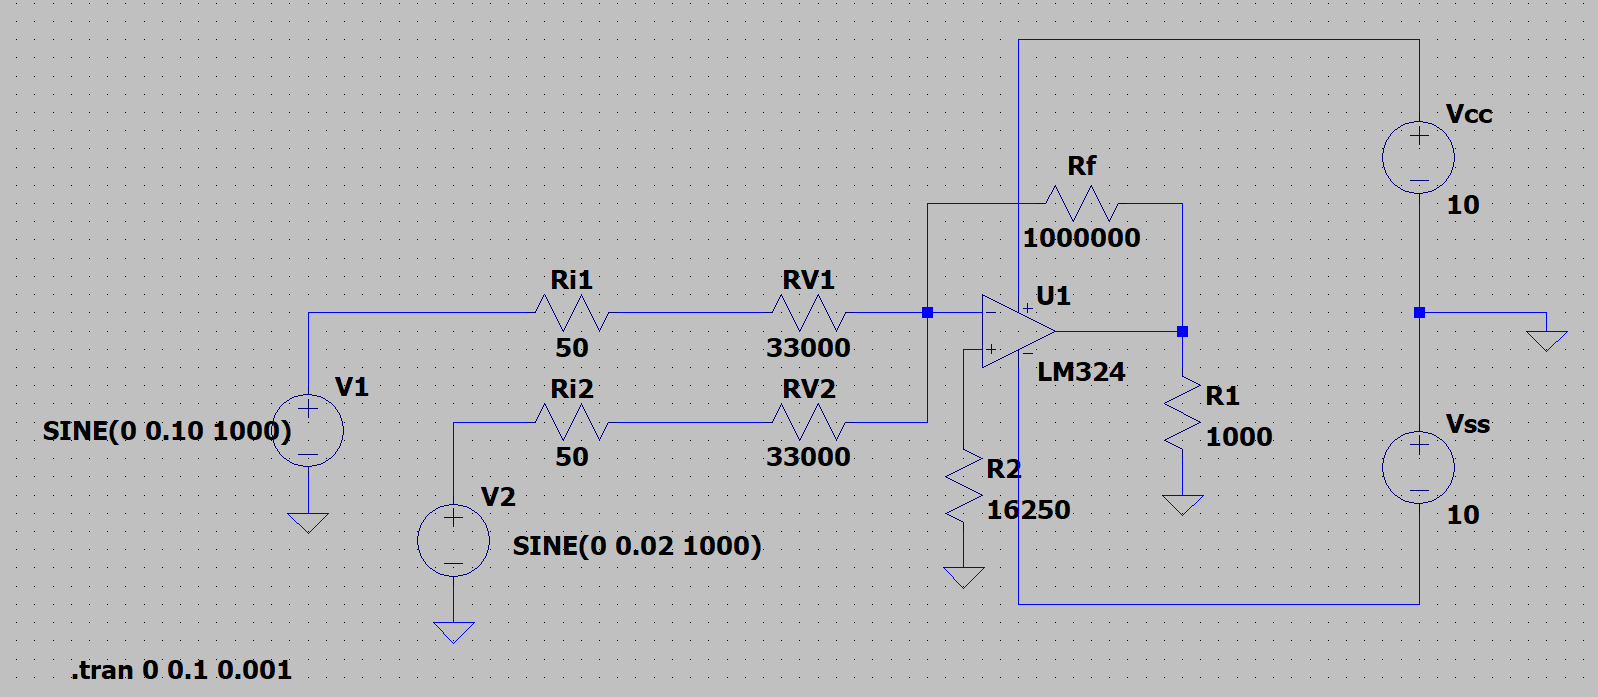
\includegraphics[width=\linewidth]{Imagenes_simulaciones/Esquematico_Circ1}
		\caption[Esquemático del circuito]{Esquemático del circuito}
		\label{fig:esquematicocirc1}
	\end{figure}
	
	\subsection{Análisis de la ganancia de tensión en la banda media}
	Aplicamos el teorema de superposición, obteniendo la ganancia de tensión respecto a una entrada anulando la otra, y luego sumando los efectos:
	
	Tanto para $V_{o}/V_{2}$ como para $V_{o}/V_{1}$ la ganancia resulta la expresión del OPAM inversor:
	\begin{equation}
		V_{o}= \frac{-Rf}{R}V1
	\end{equation}

	\begin{equation}
		V_{o}=\frac{-Rf}{R}V2
	\end{equation}
	
	La ganancia resulta:
	
	\begin{equation}
		V_{o}=\frac{-Rf}{R}(V_{1}+V_{2})
	\end{equation}
	Para obtener una ganancia aproximada de 30 veces seleccionamos las resistencias de valores comerciales con los siguientes valores $Rf=1[Mohm]$ y $R=33[Kohm]$
	
	\begin{figure}[h]
		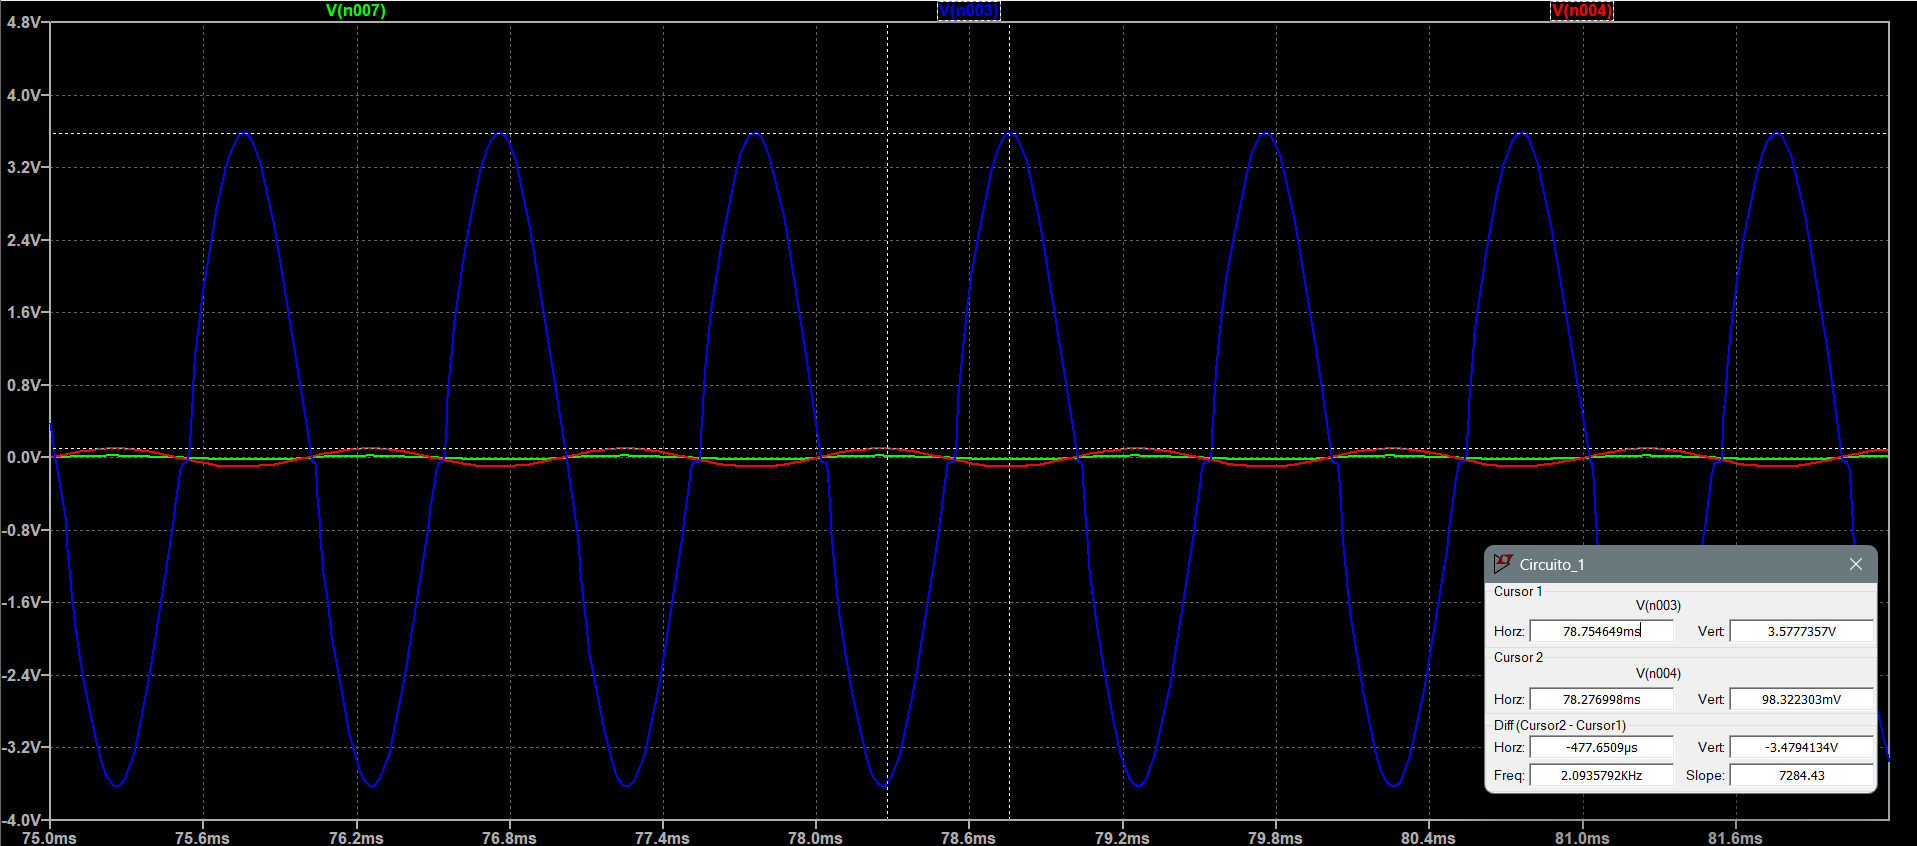
\includegraphics[width=\linewidth]{Imagenes_simulaciones/Sim_V1_0.1__V2_0.02}
		\caption[Ganancia de tensión]{Ganancia de tensión}
		\label{fig:simv10}
	\end{figure}
	
	\subsection{Análisis de errores en continua}
	Para obtener la expresión total de los errores en continua tomamos del datasheet los valores de tensión/ corriente offset, ganancia en continua a lazo abierto y RRMC:
	
	Error de corriente:
	
	\begin{equation}
		\bigtriangleup V(ipol-) =\frac{(Ipol-)(R//R//Rf)(-Ad)}{1-T}
	\end{equation}
	
	Agregamos una resistencia de ecualización en el terminal positivo para reducir el error:
	\begin{equation}
		Z=(R//R//Rf)
	\end{equation}
	\begin{equation}
			\bigtriangleup V(ipol+) =\frac{(Ipol+)(R//R//Rf)(Ad)}{1-T}
	\end{equation}

	
	\begin{equation}
		T=\frac{-R//R(Ad)}{R//R+Rf}
	\end{equation}
	
	Resultando:
	
	\begin{equation}
		\bigtriangleup V = \frac{[(Ipol+)(R//R//Rf)(Ad)]-[(Ipol-)(R//R//Rf)(-Ad)]}{1+ \frac{R//R(Ad)}{R//R+Rf}}
	\end{equation}
	
	Simplificando la expresión y teniendo en cuenta que $IOS=(Ipol+)-(Ipol-)$ tenemos:
	
	\begin{equation}
		\bigtriangleup V = \frac{(R//R//Rf)(R//R+Rf)IOS}{R//R}
	\end{equation}
	
	Con los valores de resistencias obtenidos en la sección anterior y teniendo en cuanta que la corriente de offset para el amplificador operacional LM324 es de $ 50[pA]$, el error de corriente resulta en $0.05[V]$
	
	Error de tensión:
	\begin{equation}
		\bigtriangleup V = \frac{Ad VOS}{1+\frac{R//R(Ad)}{R//R+Rf}}
	\end{equation}
	
	Simplificando la expresión:
	\begin{equation}
		\bigtriangleup V = \frac{(R//R+Rf)VOS}{R//R}
	\end{equation}
	
	Teniendo en cuenta que la tensión de offset del amplificador operacional es de $2[mV]$ el error de tension resulta en $0.123[mV]$
	
	Error de ganancia no infinita:
	\begin{equation}
		\bigtriangleup V = \frac{FS}{|T|}
	\end{equation}
	
	\begin{equation}
		\bigtriangleup V = \frac{FS}{\frac{R//R(Ad)}{R//R+Rf}}
	\end{equation}
	
	La ganancia no infinita para el LM324 es de $100dB$ el error resulta en $6.2[mV]$
	
	Error de relación de rechazo en modo común no infinita:
	En este caso tenemos el terminal positivo del amplificador operacional a masa por lo que el error de RRMC es nulo
	
	\subsection{Simulación de error en continua}
	Para aproximar cuando es el error de continua se pasivo las entradas del operacional y se mide la tensión de salida, en este caso es de $20[mV]$
	
	\begin{figure}[h!]
		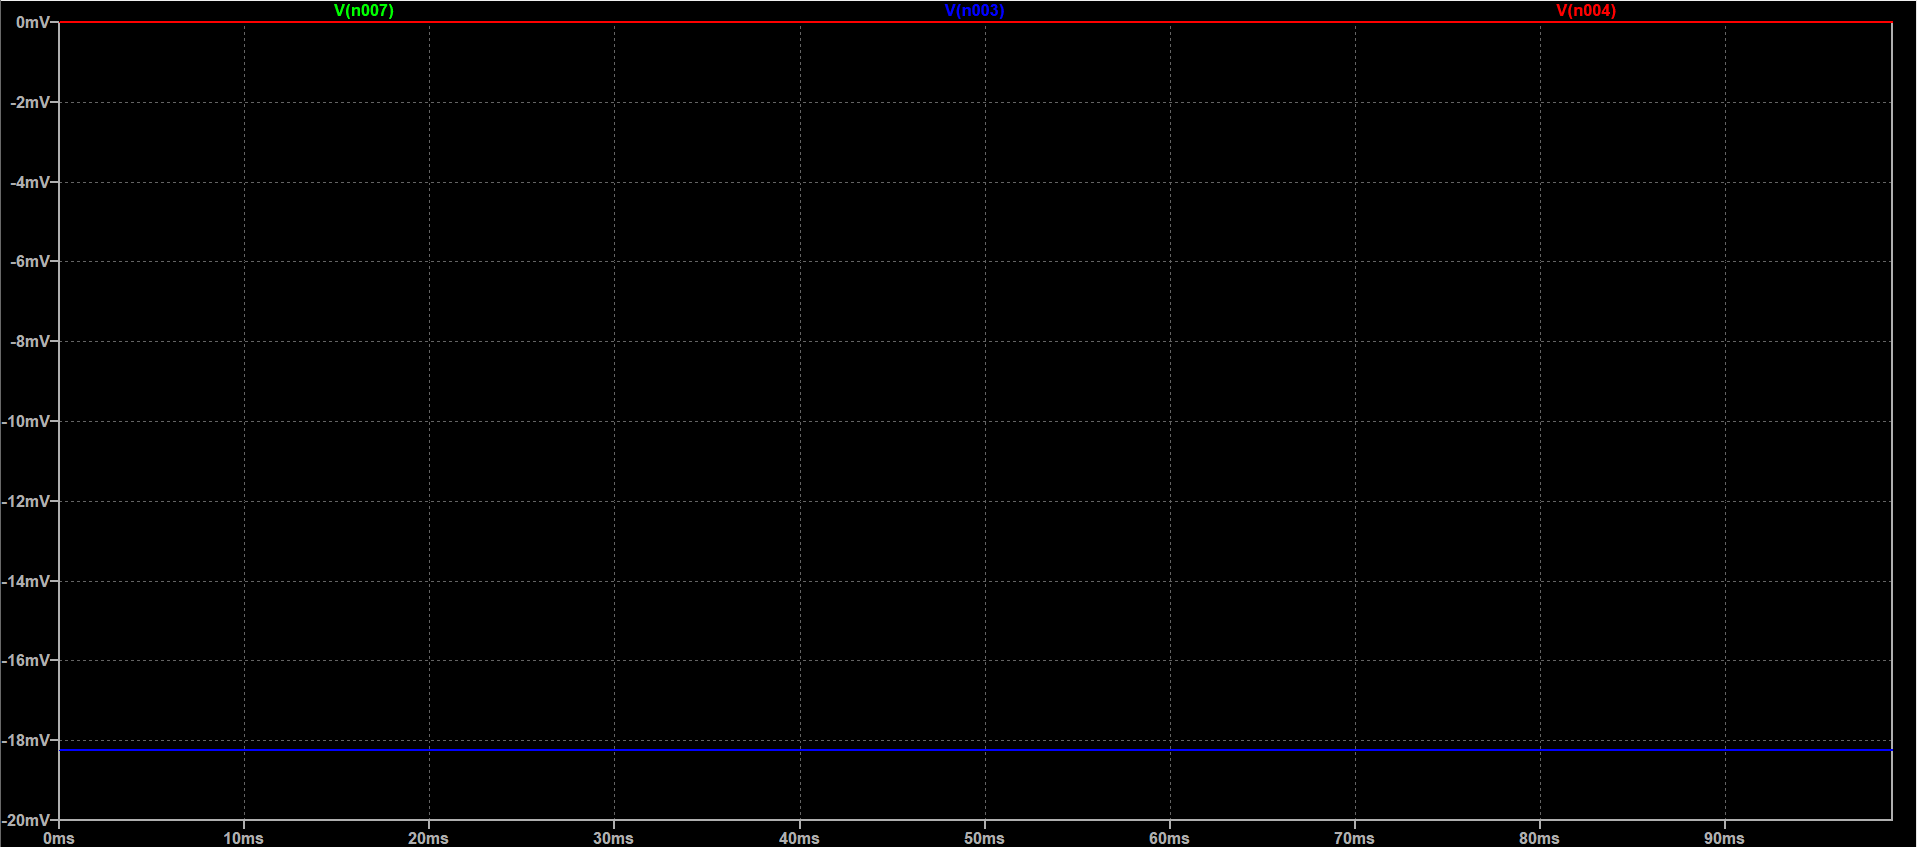
\includegraphics[width=\linewidth]{Imagenes_simulaciones/Sim_Error_DC}
		\caption[Simulación del error en DC]{Simulación del error en DC}
		\label{fig:simerrordc}
	\end{figure}
	
	\subsection{Ancho de banda de pequeña señal}
	
	\begin{equation}
		F_{H}=\frac{FT}{Avf}
	\end{equation}
	
	Teniendo en cuenta que $FT=1[MHz]$ y la ganancia a lazo cerrado es 30 tenemos que la frecuencia de corte en alta es de $F_{H}=33.3[KHz]$
	
	\begin{figure}[h!]
		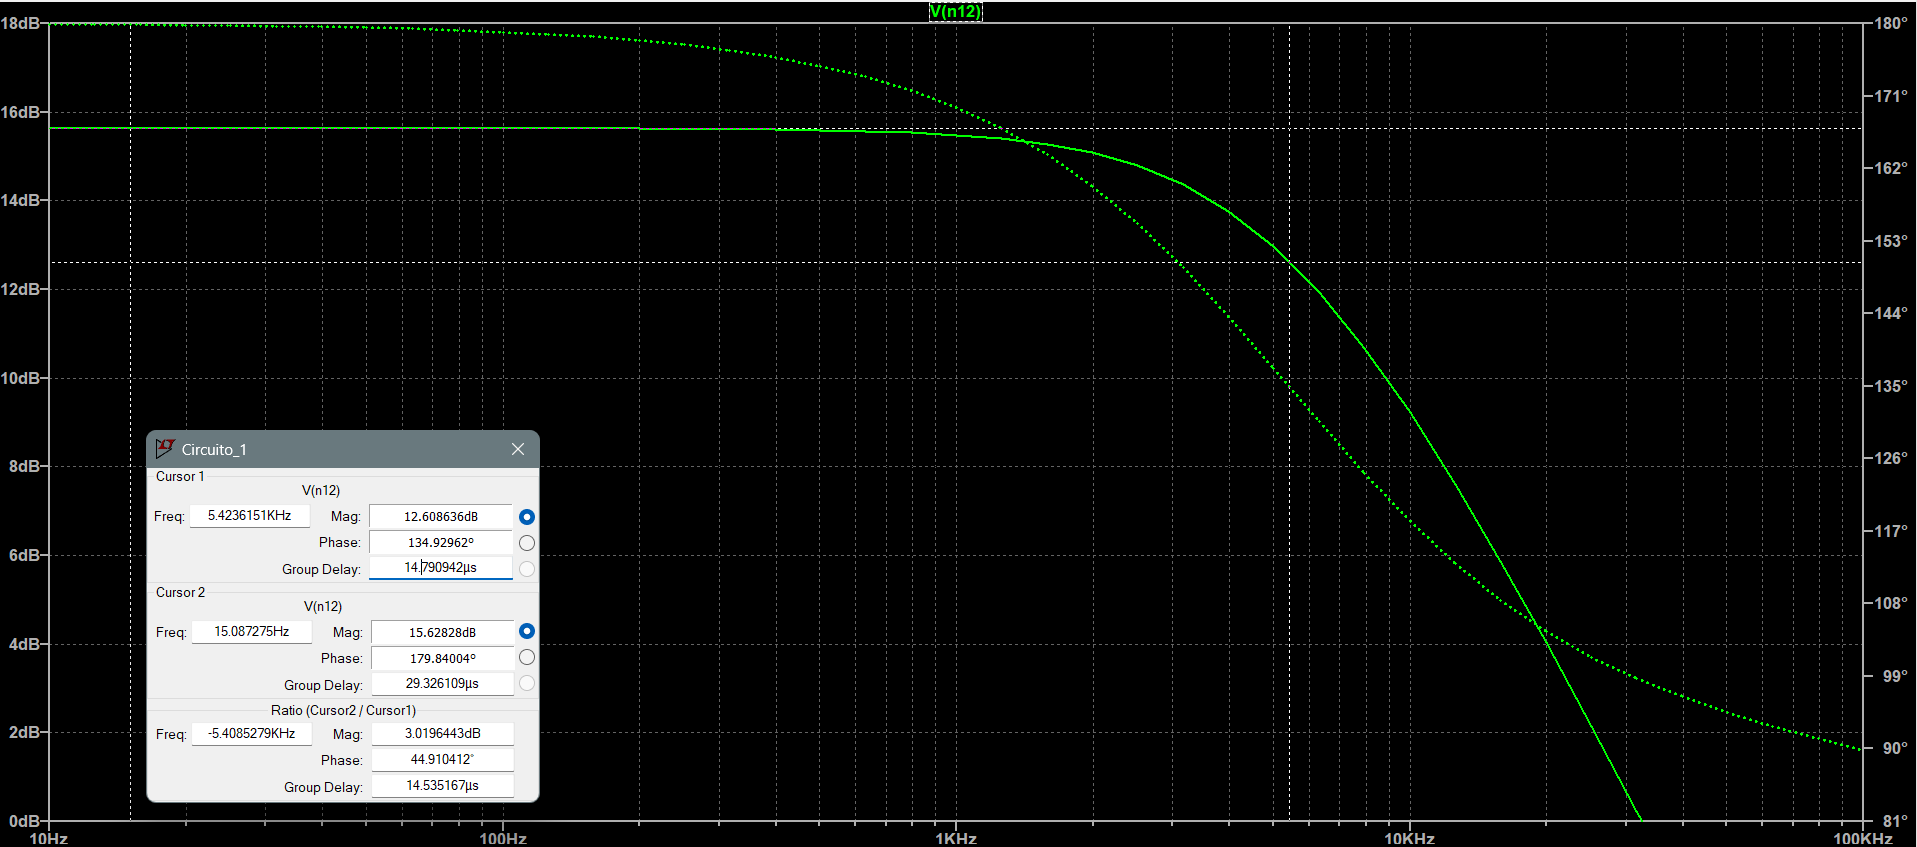
\includegraphics[width=\linewidth]{Imagenes_simulaciones/Sim_Bode_3db_marcados}
		\caption[Ancho de banda de baja señal]{Ancho de banda de baja señal}
		\label{fig:simbode3dbmarcados}
	\end{figure}

	\subsection{Ancho de banda a plena potencia}
	Para calcular el ancho de banda a plena potencia obtenemos del datasheet el valor de "slew rate" del operacional en este caso, para el LM324 es de $0.3[V/uS]$, luego:
	
	\begin{equation}
		F_[Hp]=\frac{SR}{2\pi FS} = 4775[Hz]
	\end{equation} 
	
	\begin{figure}[h!]
		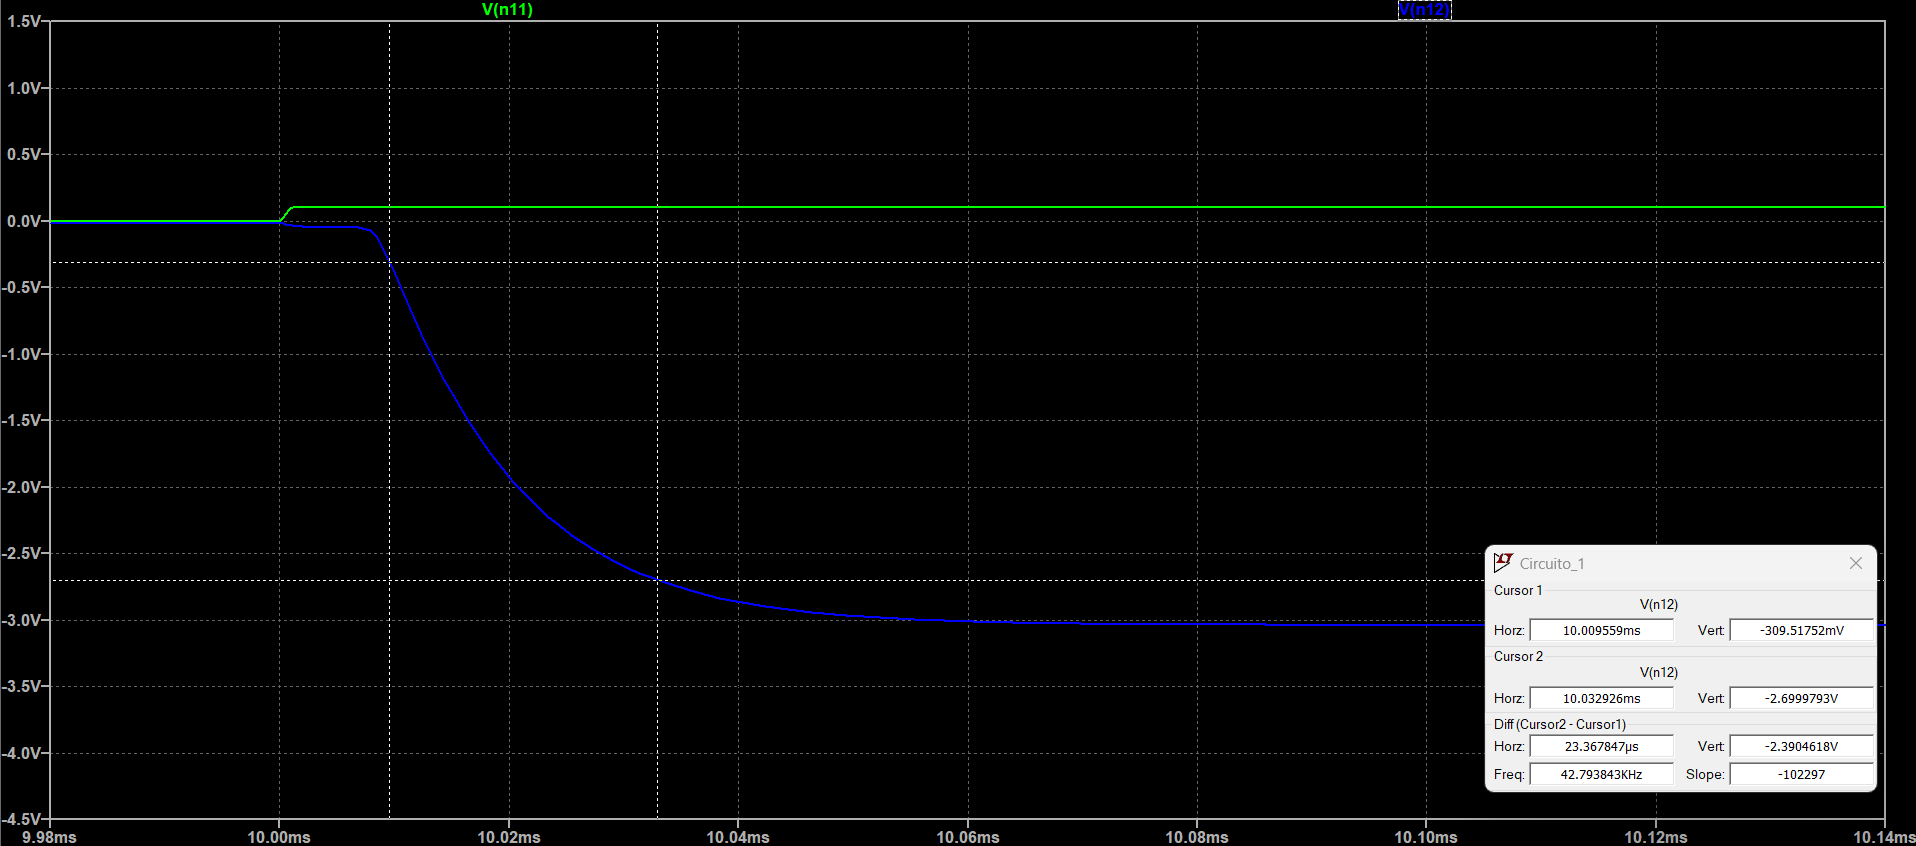
\includegraphics[width=\linewidth]{Imagenes_simulaciones/Sim_slow_rate}
		\caption[Slew rate]{Slew rate}
		\label{fig:simslowrate}
	\end{figure}
	
	\section{Circuito II: Amplificadores en cascada con puente de  Wheatstone }
	En este circuito tenemos un puente de Wheastone que produce una tensión diferencial, esta se amplifica mediante dos etapas, una no inversora (primera) y otra no inversora (segunda).
	
	\subsection{Análisis de la ganancia de tensión en la banda media}
	Para la primera etapa tenemos amplificador en configuración no inversora, la ganancia resulta:
	\begin{equation}
		\frac{Vx}{Vin}=(1+\frac{R1}{aR1})
	\end{equation}
	
	Teniendo en cuenta que $aR1=47[Kohm]$ y $R1=2.2[Kohm]$, la ganancia resulta: $1.046$
	
	Para la segunda etapa tenemos un inversor donde la ganancia de tensión resulta:
	\begin{equation}
		\frac{Vo}{Vx}= \frac{-aR2}{R2}
	\end{equation}
	
	Teniendo en cuenta que $aR2=47[Kohm]$ y $R2=2.2[Kohm]$, la ganancia resulta: $-21.36$
	Por lo tanto la ganancia resultante es de $-22.34$, aproximadamente.
	
	\begin{figure}
		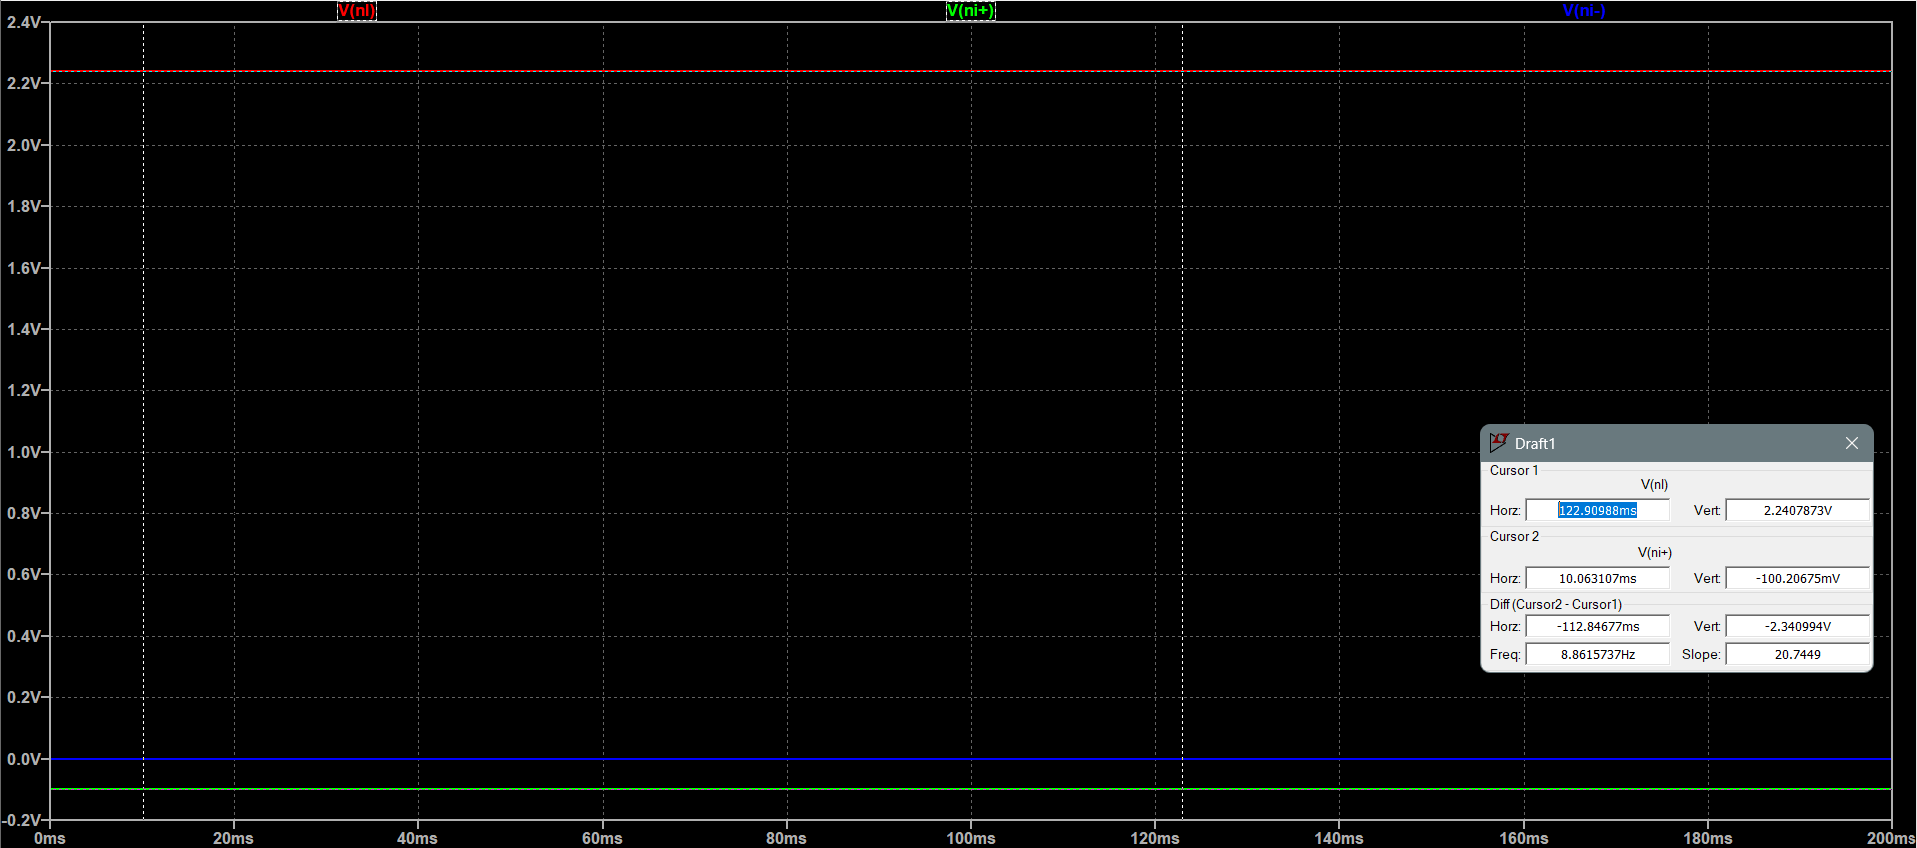
\includegraphics[width=\linewidth]{Imagenes_simulaciones/Sim_Ganancia_C2}
		\caption[Ganancia de tensión en la banda media]{Ganancia de tension en la banda media}
		\label{fig:simgananciac2}
	\end{figure}
	
	\subsection{Análisis de error en continua}
	Error de corriente del primer amplificador:
	
	\begin{equation}
		V(Ipol+)=\frac{(Ipol+)(Rp//Rp)(Ad)(-aR2/R2)}{(1-T1)}
	\end{equation}
	\begin{equation}
		V(Ipol-)=\frac{(Ipol-)(aR1//R1)(-Ad)(-aR2/R2)}{(1-T1)}
	\end{equation}
	\begin{equation}
		T1=\frac{-aR1(Ad)}{R1}
	\end{equation}
	
	Simplificando la expresión queda:
	\begin{equation}
		\bigtriangleup V= \frac{(Ipol)(-aR2/R2)[aR1//R1-Rp//Rp]}{\frac{aR1}{R1}}
	\end{equation}
	
	Reemplazando los valores de las resistencias y conociendo el valor de la corriente de polarización del amplificador operacional, $Ipol=90[nA]$, el error de corriente para la primera etapa es de $40.04[uV]$
	
	Error de corriente del segundo amplificador:
	\begin{equation}
		V(Ipol+)=\frac{(Ipol+)(Rp//Rp)(Ad)}{(1-T2)}
	\end{equation}
	\begin{equation}
		V(Ipol-)=\frac{(Ipol-)(aR2//R2)(-Ad)}{(1-T2)}
	\end{equation}
	\begin{equation}
		T2=\frac{-R2(Ad)}{aR2}
	\end{equation}
	
	Simplificando la expresión queda:
	\begin{equation}
		\bigtriangleup V= \frac{(Ipol)[(Rp//Rp)-(R2//aR2)]}{\frac{R2}{aR2}}
	\end{equation}
	
	El error de corriente para el segundo operacional resulta $0.86[mV]$
	
	Error de tensión de offset para el primer operacional
	\begin{equation}
		\bigtriangleup V = \frac{VOS(aR2//R2)}{\frac{aR1}{R1}}
	\end{equation}
	
	Para una tensión de offset de  $2[mV]$  el error resulta $2[mV]$
	
	Error de tensión para el segundo operacional
	\begin{equation}
		\bigtriangleup V=\frac{VOS}{\frac{R2}{aR2}}
	\end{equation}
	Error resulta $42.7[mV]$
	
	Error de ganancia no infinita:
	\begin{equation}
		\bigtriangleup V = \frac{FS}{|T1|}=2.36[uV]
	\end{equation}
	
		\begin{equation}
		\bigtriangleup V = \frac{FS}{|T2|}=1.068[mV]
	\end{equation}
	
	\begin{figure}
		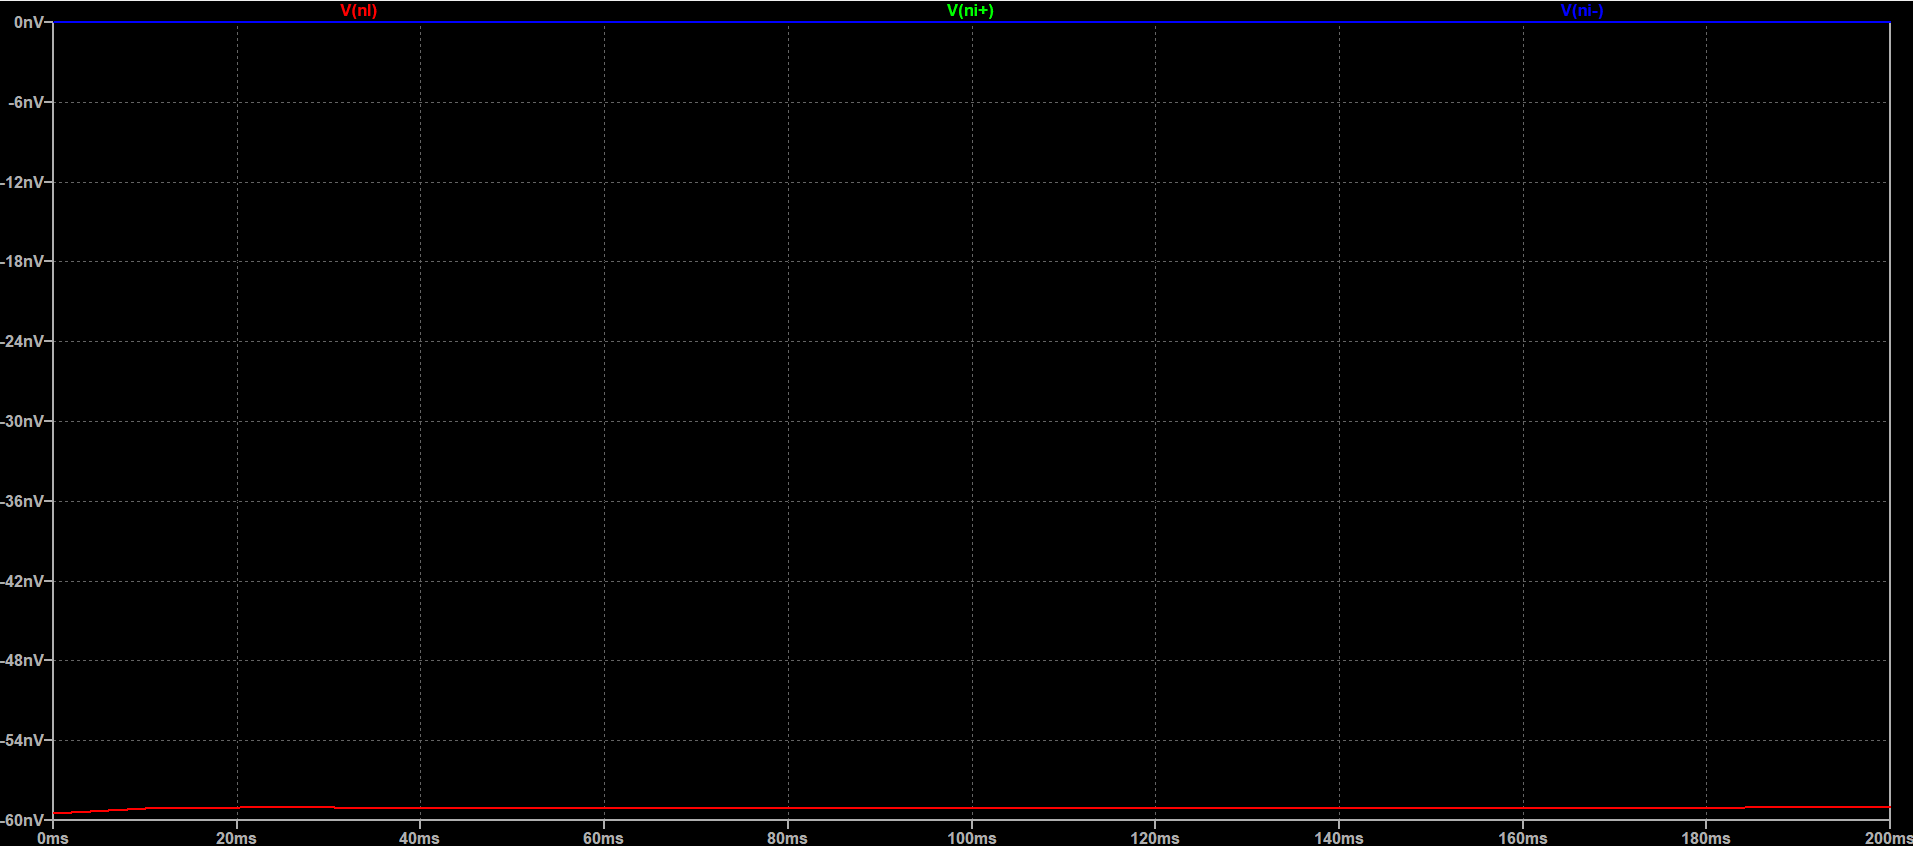
\includegraphics[width=\linewidth]{Imagenes_simulaciones/Sim_Error_DC_C2}
		\caption[Error en DC]{Error en DC}
		\label{fig:simerrordcc2}
	\end{figure}
	
	El error total en continua resulta: $46.6[mV]$, calculamos la resolución en bits para el ADC:
	\begin{equation}
		\bigtriangleup V <= \frac{FE}{2^n}
	\end{equation}
	
	\begin{equation}
		n = \log(\frac{FS}{\bigtriangleup V}) = 6.74 bits
	\end{equation}
	
\end{document}
}